\documentclass[12pt]{article}

\usepackage{graphicx}% Include figure files
\usepackage{dcolumn}% Align table columns on decimal point

% Use Arial font %
\usepackage{helvet}
\renewcommand{\familydefault}{\sfdefault} 

% Default margins and paper properties %
\usepackage[a4, portrait, margin=0.6in]{geometry}

\begin{document}
	\title{Hypothesis plots summary} % Force line breaks with \\
	\author{1666957, Gustavo Espinal Lugo}
	\date{\today} % It is always \today, today, %  but any date may be explicitly specified

	\maketitle
	%\tableofcontents
	
	\section*{Plots and corresponding metadata}
	Number of data points used: 99999,\\
mean expected W mass: 80.36010913 $[GeV/c^{2}]$,\\
mean hypothesis masses $[GeV/c^{2}]$: [<generator object <genexpr> at 0x7f755dc85510>],\\
mass width: 2.07041274 $[GeV/c^{2}]$,\\
chi\_square value of hypothesis fit: 4.4227748580892285\\
	Absolute path to figure: /home/physics/phuxdp/Desktop/PX402 Physics Project/WBosonProject/noQED/plots/muPT\_80.36010913\_2.07041274\_between\_78\_and\_82.png\\
	Next lines are the data of the shown histograms (if needed): \\
	All quantities: 	99999, 80.36010913, [78.  78.5 79.  79.5 80.  80.5 81.  81.5 82. ], 2.07041274, 4.4227748580892285\\
	X\_energ\_vls = [30.1, 30.299999999999997, 30.5, 30.700000000000003, 30.9, 31.1, 31.299999999999997, 31.5, 31.700000000000003, 31.9, 32.1, 32.3, 32.5, 32.7, 32.9, 33.1, 33.3, 33.5, 33.7, 33.9, 34.1, 34.3, 34.5, 34.7, 34.9, 35.1, 35.3, 35.5, 35.7, 35.9, 36.1, 36.3, 36.5, 36.7, 36.9, 37.1, 37.3, 37.5, 37.7, 37.9, 38.1, 38.3, 38.5, 38.7, 38.9, 39.1, 39.3, 39.5, 39.7, 39.9, 40.1, 40.3, 40.5, 40.7, 40.9, 41.1, 41.3, 41.5, 41.7, 41.9, 42.1, 42.3, 42.5, 42.7, 42.9, 43.1, 43.3, 43.5, 43.7, 43.9, 44.1, 44.3, 44.5, 44.7, 44.9, 45.1, 45.3, 45.5, 45.7, 45.9, 46.1, 46.300000000000004, 46.5, 46.7, 46.9, 47.1, 47.300000000000004, 47.5, 47.7, 47.9, 48.1, 48.300000000000004, 48.5, 48.7, 48.9, 49.1, 49.300000000000004, 49.5, 49.7, 49.9]\\
	Y\_data\_bin\_cnts = [266.0, 281.0, 301.0, 304.0, 281.0, 321.0, 336.0, 324.0, 300.0, 328.0, 328.0, 325.0, 318.0, 337.0, 328.0, 371.0, 345.0, 331.0, 383.0, 356.0, 327.0, 345.0, 368.0, 354.0, 369.0, 369.0, 367.0, 344.0, 389.0, 342.0, 384.0, 374.0, 371.0, 385.0, 365.0, 370.0, 364.0, 348.0, 351.0, 340.0, 420.0, 408.0, 389.0, 399.0, 403.0, 398.0, 377.0, 376.0, 348.0, 319.0, 320.0, 307.0, 319.0, 305.0, 286.0, 320.0, 272.0, 260.0, 239.0, 235.0, 228.0, 215.0, 216.0, 211.0, 204.0, 180.0, 196.0, 185.0, 158.0, 154.0, 148.0, 127.0, 134.0, 128.0, 120.0, 120.0, 123.0, 101.0, 104.0, 94.0, 110.0, 105.0, 81.0, 79.0, 100.0, 86.0, 75.0, 76.0, 86.0, 83.0, 80.0, 77.0, 65.0, 70.0, 73.0, 61.0, 64.0, 56.0, 57.0, 66.0]\\
	Y\_model\_bin\_cnts = [276.93023681640625, 266.4456481933594, 268.41180419921875, 283.21356201171875, 284.0470275878906, 251.14630126953125, 325.6341552734375, 274.7048645019531, 271.8363037109375, 305.3310546875, 299.5513000488281, 274.57220458984375, 288.62127685546875, 270.2326354980469, 267.7138366699219, 396.50494384765625, 294.8599853515625, 357.4852600097656, 338.5548095703125, 358.7528076171875, 330.4515075683594, 344.71673583984375, 299.2892150878906, 299.9137268066406, 317.0308532714844, 363.6265869140625, 298.5186767578125, 328.7791442871094, 386.07647705078125, 305.718994140625, 322.8080139160156, 350.8438720703125, 341.25885009765625, 408.4336242675781, 371.0982666015625, 394.10107421875, 290.3528747558594, 374.34332275390625, 342.9143371582031, 393.4912109375, 356.8514404296875, 368.5692138671875, 374.96185302734375, 378.3891906738281, 385.7430725097656, 365.4502868652344, 384.804931640625, 379.839111328125, 320.8994445800781, 307.15509033203125, 356.5126953125, 332.96112060546875, 347.9140319824219, 318.1734619140625, 339.9112243652344, 341.9465026855469, 278.9992980957031, 242.48016357421875, 269.8632507324219, 270.4671936035156, 220.29945373535156, 180.79222106933594, 251.67237854003906, 194.96792602539062, 191.2952117919922, 217.257080078125, 208.83395385742188, 178.58535766601562, 196.30352783203125, 184.05862426757812, 155.99424743652344, 192.88046264648438, 163.90553283691406, 142.6587371826172, 161.1498565673828, 109.65188598632812, 106.79487609863281, 112.27214050292969, 120.26044464111328, 67.11335754394531, 90.34393310546875, 118.6343765258789, 92.7890396118164, 130.8133544921875, 91.84986877441406, 86.48822784423828, 90.47335052490234, 90.51984405517578, 98.55259704589844, 80.27766418457031, 58.94035720825195, 42.623714447021484, 73.8402328491211, 68.56688690185547, 69.27615356445312, 55.036808013916016, 65.38597106933594, 90.8377914428711, 58.06388854980469, 54.15039825439453]\\

    Found optimal massses ($\chi^2$ roots): [80.46716523] $[GeV/c^{2}]$\\
    Uncertainty [GeV/c^2]: 1.4210854715202004e-14\\

	\begin{figure}[tb]
		\centering
		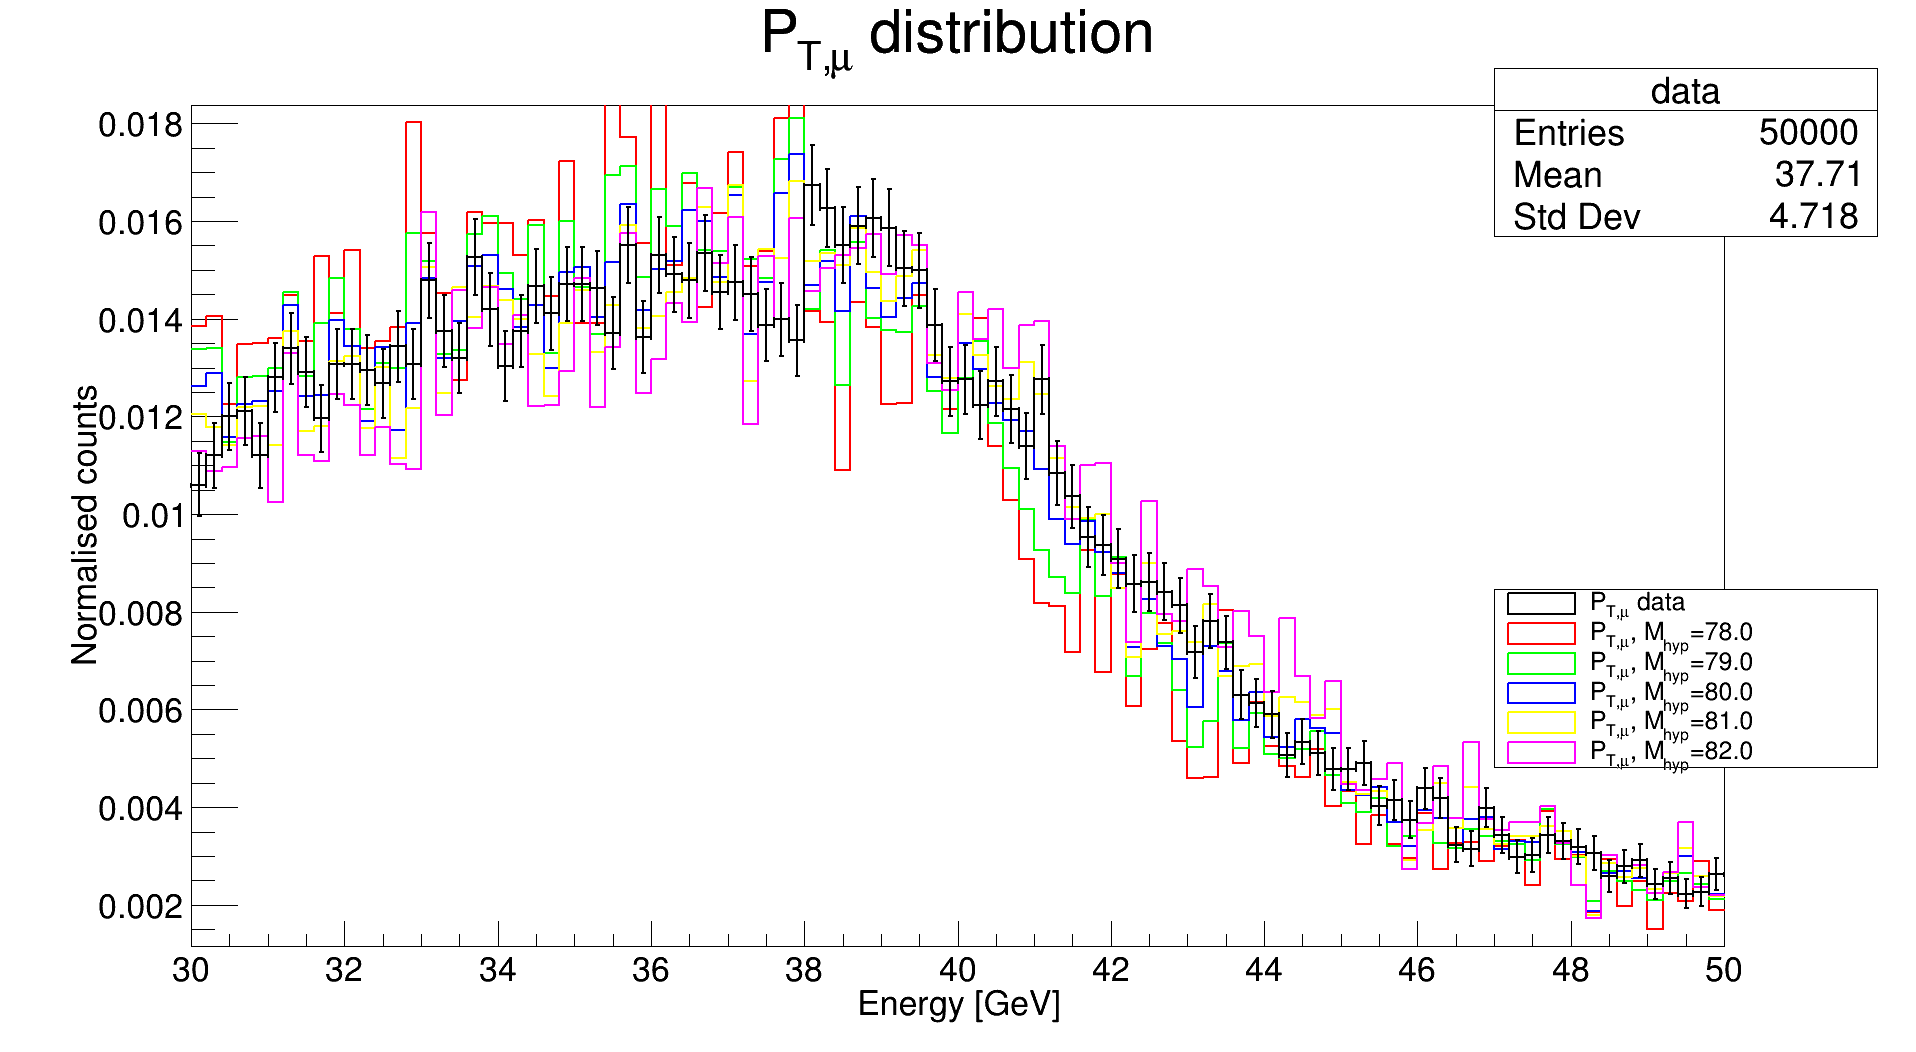
\includegraphics[width=\columnwidth]{/home/physics/phuxdp/Desktop/PX402 Physics Project/WBosonProject/noQED/plots/muPT_80.36010913_2.07041274_between_78_and_82.png}
		\caption{\small Hypothesis masses Number of data points used: 99999,\\
mean expected W mass: 80.36010913 $[GeV/c^{2}]$,\\
mean hypothesis masses $[GeV/c^{2}]$: [<generator object <genexpr> at 0x7f755dc85510>],\\
mass width: 2.07041274 $[GeV/c^{2}]$,\\
chi_square value of hypothesis fit: 4.4227748580892285. }
		\label{fig: fig_0}
	\end{figure}
    Notes: \\
    1) Using mu\_born\_PT as pseudodata and  Mu\_Pt as model/hypothesis\\
    2) Using full run mode\\
       \begin{figure}[tb]
		\centering
		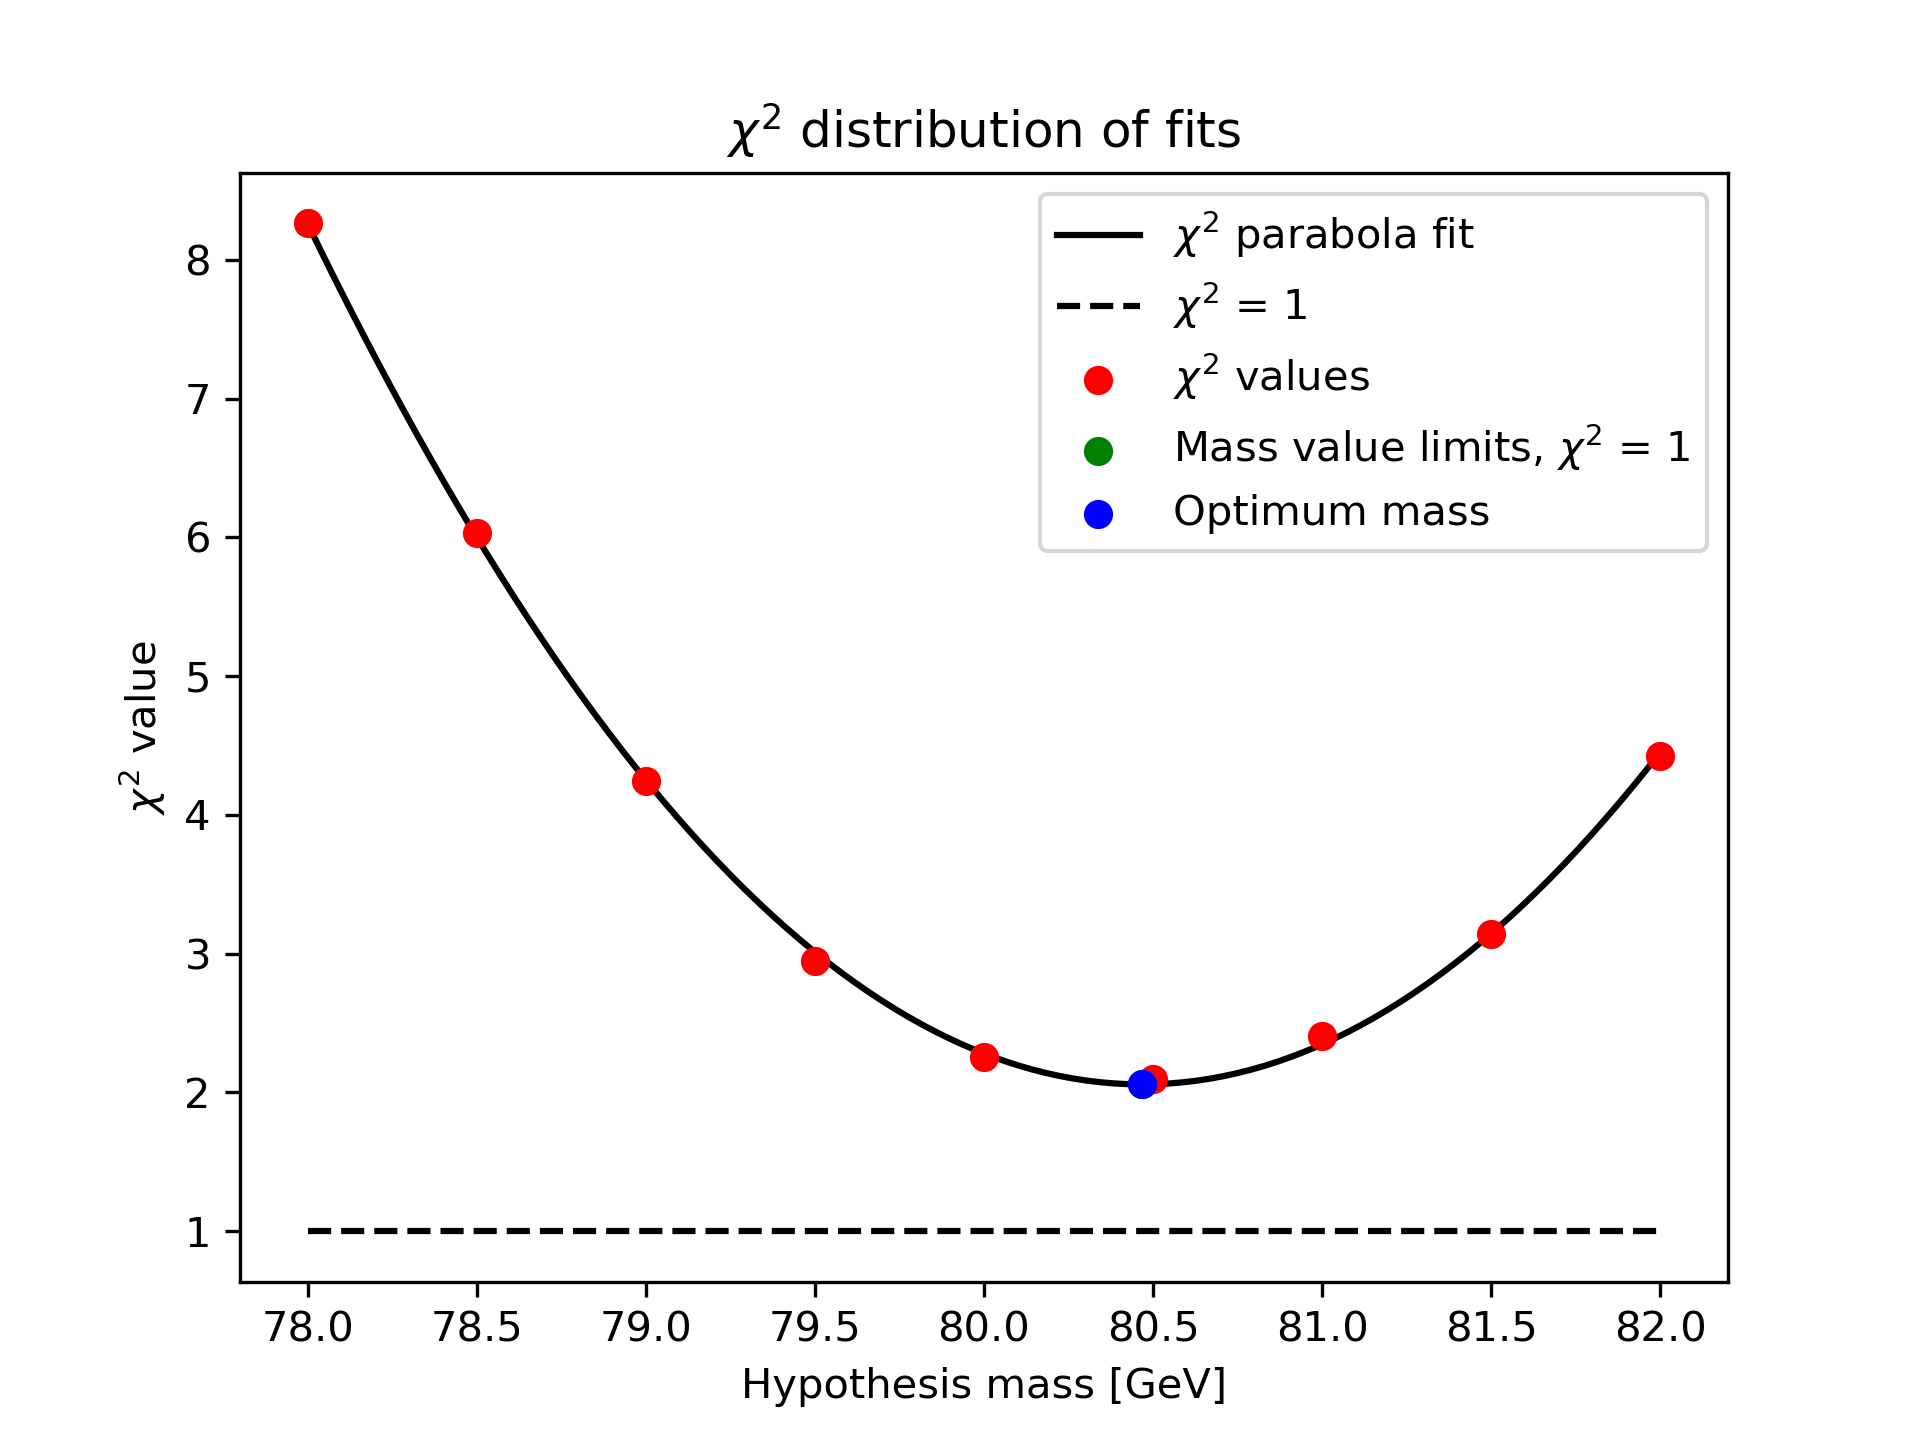
\includegraphics[width=\columnwidth]{/home/physics/phuxdp/Desktop/PX402 Physics Project/WBosonProject/noQED/plots/chi_square_fits_muPT_80.36010913_2.07041274_between_78_and_82.png}
		\caption{\small $\chi^2$ of hypothesis masses. }
		\label{fig: fig_chi_square}
	\end{figure}

    \begin{figure}[tb]
		\centering
		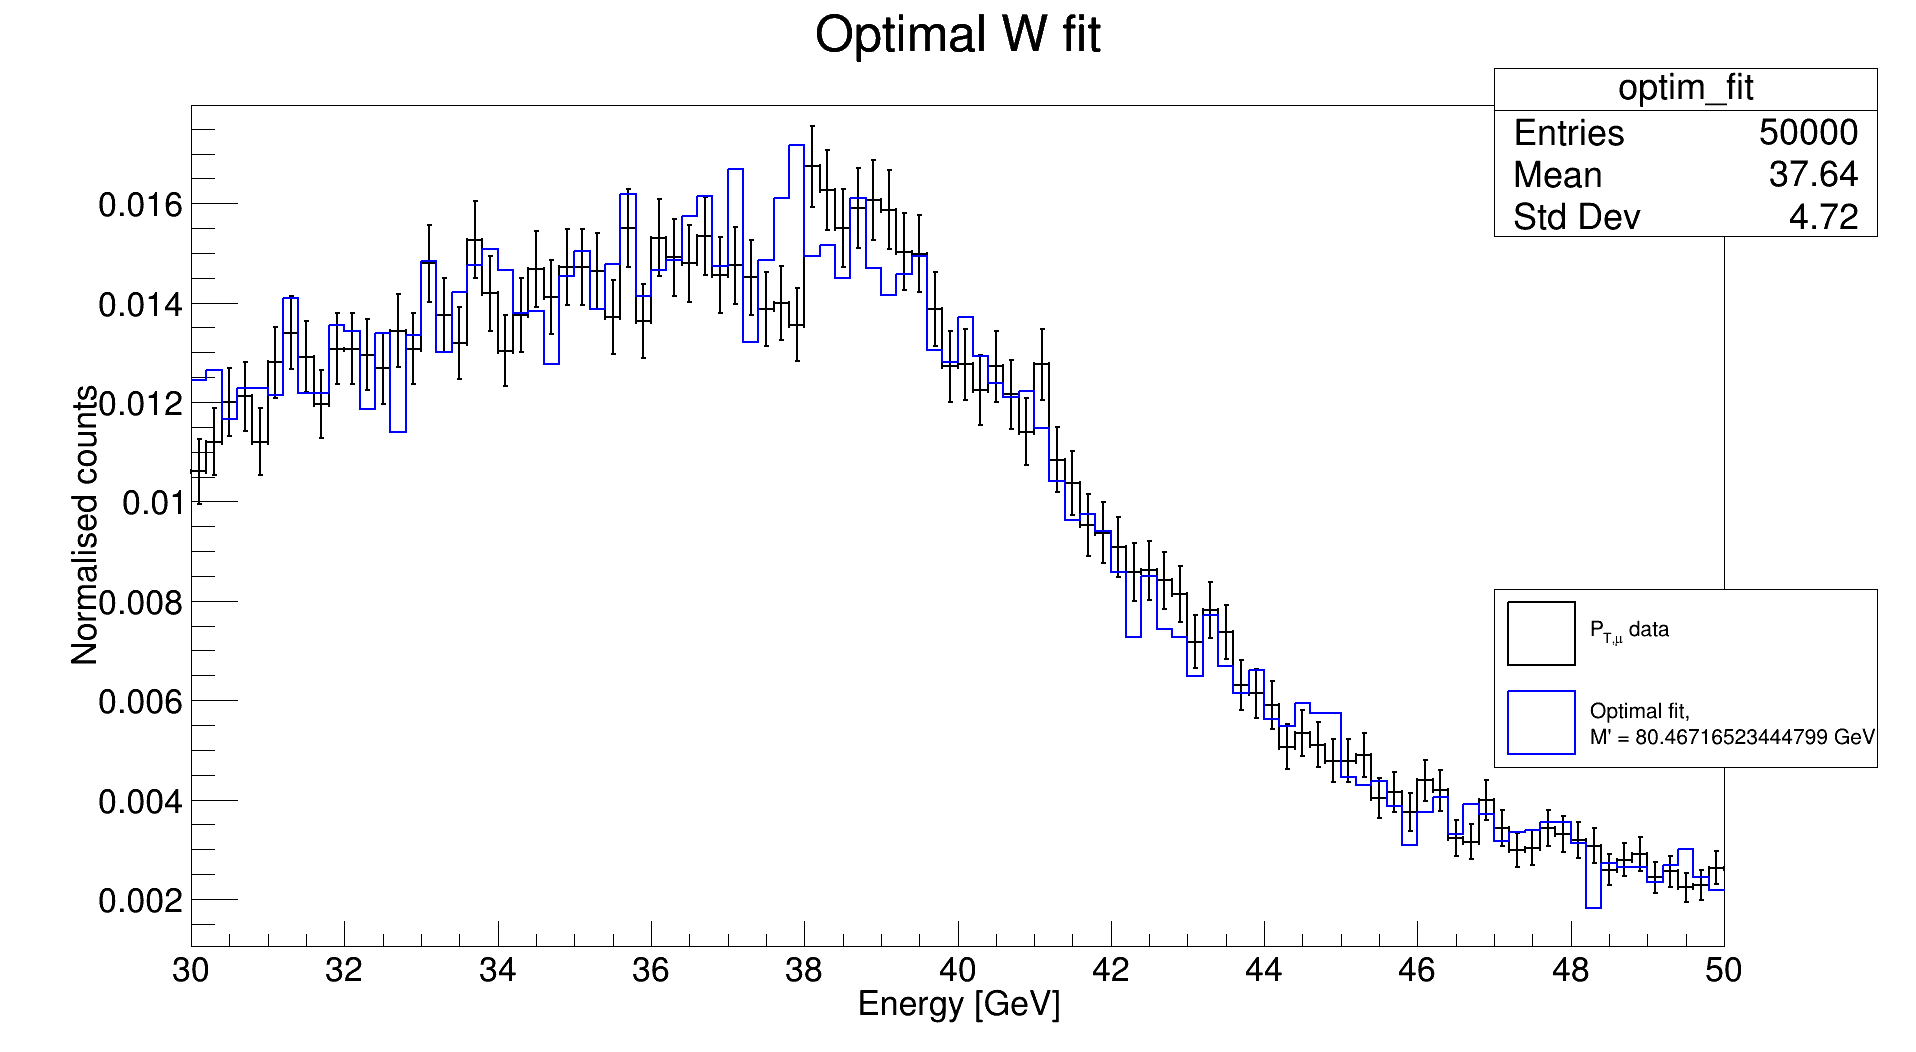
\includegraphics[width=\columnwidth]{/home/physics/phuxdp/Desktop/PX402 Physics Project/WBosonProject/noQED/plots/optimum_muPT_80.36010913_2.07041274_between_78_and_82.png}
		\caption{\small Data and optimum fit with $\chi^2 = 2.1689569886085476$. Used the hypothesis mass of 80.46716523444799 $[GeV/c^{2}]$. }
		\label{fig: fig_optim_parms}
	\end{figure}
    
\end{document}